\documentclass[12pt]{report}

%------------------- declaring packages---------------------------------


% styling and graphics-based
\usepackage{url}
\usepackage{graphicx} 
\usepackage{emptypage}
\usepackage{geometry}
\usepackage{setspace}
\usepackage{pgf}
\usepackage{pgffor}
\doublespacing

% for figures and tables

% figures:
\usepackage{subfigure}  
\usepackage{adjustbox}
\usepackage{wrapfig}
\usepackage{subfigure}
\usepackage{rotating}
\usepackage{lscape}
% tables:
\usepackage{tabularx,ragged2e,booktabs,caption}
\usepackage{multicol,tabularx,capt-of}
\usepackage{hhline}
\usepackage{multirow}
\usepackage{array}


% for math equations

\usepackage{amssymb}
\usepackage{float}
\usepackage{verbatim}
\usepackage{amsmath} 
\usepackage{amsthm}   


% for acronyms and glossaries

\usepackage{acronym}
\usepackage{glossaries}


% for hyperlinks

\usepackage[round]{natbib}
\usepackage[colorlinks = true,
            linkcolor = blue,
            urlcolor  = blue,
            citecolor = blue,
            anchorcolor = blue]{hyperref}

\usepackage{sectsty}
\allsectionsfont{\bfseries}
\chapterfont{\centering\Large}
\sectionfont{\normalsize}
\subsectionfont{\normalsize}


\usepackage [english]{babel}
\usepackage [autostyle, english = american]{csquotes}
\MakeOuterQuote{"}



% header formatting



%footer formatting

\interfootnotelinepenalty=10000 

\usepackage{epstopdf}
\usepackage{lipsum} 

%----------------------------begin document-------------------------------


\begin{document}
\begin{titlepage}

\end{titlepage}

%\frontmatter
\pagenumbering{roman}

\chapter*{Abstract}
This project presents the development of a Personal Financial Dashboard aimed at enhancing financial management and decision-making skills. Leveraging Power BI as the primary tool, the dashboard aggregates and visualizes individual financial data, offering insights into income, expenses, and overall financial health. Through a user-centered design approach, the dashboard provides a user-friendly interface, enabling users to track their financial activities comprehensively. The iterative development process addressed challenges in data management, visualization design, and user experience, resulting in an intuitive and impactful financial management tool. This project underscores the importance of financial literacy and empowerment in personal finance and demonstrates the potential of personal financial dashboards in facilitating informed financial decision-making.
\\\
\vspace{1cm}
\textbf{Keywords: }{Personal Financial Dashboard, Power BI. }

\tableofcontents{}

\listoffigures{}

\chapter*{Acronyms}
\thispagestyle{noheaderfooter}

\begin{acronym}

% list down all your acros here


  \acro{BI}{Business Intelligence}
  \acro{DAX}{Data Analysis Expressions}




\end{acronym}



 





%%%%%%%%%%%%%%%%%%%%%%%%%%%%%%%%%%%%%%%%%%%%%%%%%%%%%%%%%%%%%%%%ù 
\pagenumbering{arabic}
\chapter*{Introduction}

\textbf{Statement of the Problem}

The lack of effective tools for personal financial management poses a significant challenge for individuals seeking to achieve financial stability and secure their future. Without a comprehensive system in place, many individuals struggle to track their income, expenses, and savings effectively, leading to financial stress and uncertainty.
\textbf{Objectives}

The primary objective of this project is to address the aforementioned challenge by developing a Personal Financial Dashboard. This tool aims to empower individuals to take control of their finances by providing a user-friendly platform for organizing, analyzing, and visualizing their financial data. Specifically, the objectives of the project include:

\begin{itemize}
   
     \item Designing and implementing a dashboard interface for tracking income, expenses, and savings.
     \item Providing users with insights into their financial habits and patterns through data visualization.
     \item Improving financial literacy and decision-making skills through the use of informative dashboards.
    \item Enhancing user experience and usability to ensure accessibility for individuals of all levels of financial expertise.
\end{itemize}


    

\chapter{Introduction}
\label{ch1}

 %%%%%%%%%%%%%%%%%%%%%% POWER BI %%%%%%%%%%%%%%%%%%%%%ù
\section{Power BI}

\begin{figure}[h]
    \centering
    
\includegraphics[width=2.0in, height=2.0in]{Figure/power bi.jpg}
    \caption{Power BI }
    \label{fig:enter-label}
\end{figure}

Power BI is a business analytics service provided by Microsoft. It aims to provide interactive visualizations and business intelligence capabilities to create their own reports and
dashboards for the end users. Our data may be in an Excel spreadsheet, or a collection of a cloud based .Pbix file which is designed for to use with Power BI desktop.
\\ 
Power BI was initially released in 2014, operating system: Microsoft windows. It provides cloud- based services, along with desktop interface, called Power BI Desktop. The key components of the Power BI are (The first one was used in this project): 
\begin{itemize}
    \item Power BI desktop: designing and publishing reports and dashboards to the service.
    \item Power BI service: software as a service.
    \item Power BI mobile apps: iOS, android, and windows phones.
\end{itemize}
Power BI is used for data visualization, analysis, and reporting. It enables users to transform raw data into interactive and visually appealing dashboards and reports, allowing organizations to gain insights and make data-driven decisions.

%%%%%%%%%%%%%%%%%%%%%%% USE CASES %%%%%%%%%%%%%%%%%%%%%%%%
\subsection{Power BI use cases}
The platform's ability to synthesize data from various sources makes it useful for analyzing and reporting data that's culled using an array of tools and methods. Some of the ways different industry sectors use Power BI to their advantage include the following:
\begin{enumerate}
    \item \textbf{Retail:} Reports based on customer purchase data give retailers insight into which products to prioritize and stock.
    \item \textbf{Manufacturing and engineering:} Power BI dashboards are used for process monitoring and reporting resource use. For instance, manufacturing data collected with IoT devices can be analyzed using Power BI. \\
    \item \textbf{Education:} Tracking student performance with Power BI reports and dashboards helps school administrators and teachers identify where improvements are needed.
    \item \textbf{Finance and insurance:} Power BI is conducive to analyzing the large-scale data sets the financial sector uses. The insurance industry can use reports and dashboards to get insight into risk assessments.
\end{enumerate}

%%%%%%%%%%%%%%%%%%%%%%% flow process %%%%%%%%%%%%%%%%%%%%%%%
\subsection{Understanding the Process Flow in Power BI}

\begin{figure}[h]
    \centering
    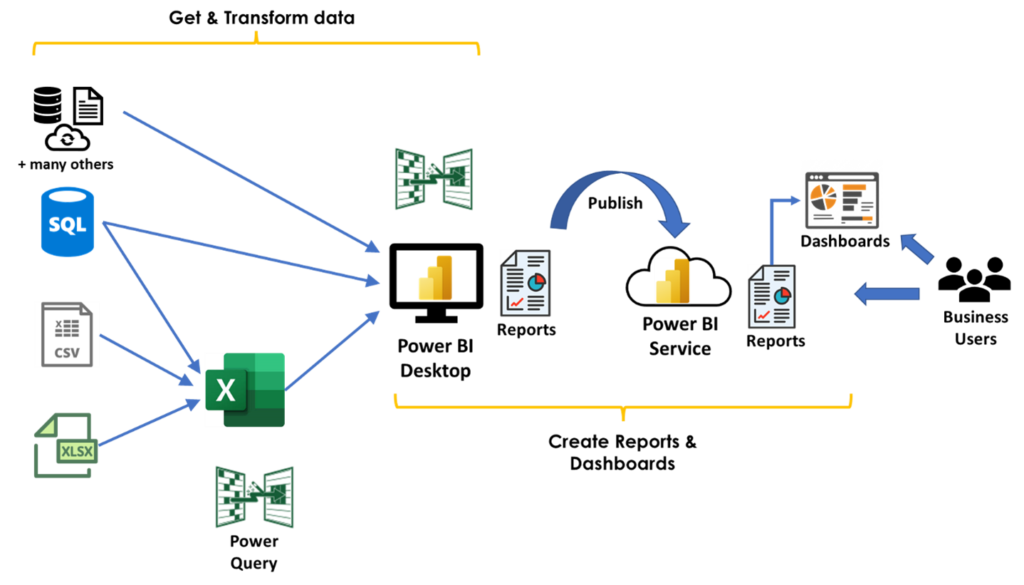
\includegraphics[width=5.0in, height=3.0in]{Figure/Power_BI_Process.png}
    \caption{Process flow in power BI }
    \label{fig:enter-label}
   \textit{Source:} \href{https://sqlspreads.com/blog/power-bi-dashboards-examples-use-cases/}{sqlspreads.com}
\end{figure}

The process flow in Power BI involves several key steps. Initially, data is collected from diverse sources such as databases, spreadsheets, and web services. This data is then transformed, cleaned, and prepared for analysis. Users define relationships between different data tables to create data models that serve as the foundation for analysis. With the data model in place, interactive reports and dashboards are created to visualize the data effectively. Users can then analyze the data to uncover insights, trends, and patterns. These insights can be shared with colleagues and stakeholders for collaborative decision-making. Finally, Power BI solutions are deployed and managed in a production environment to ensure scalability and reliability.

%%%%%%%%%%%%%%%%%%%%%%%% ADV / DIS %%%%%%%%%%%%%%%%%%%%%%%%



%%%%%%%%%%%%%%%%%%%%%%%% Benifits of power bi dash %%%%%%%%%%%%
\section{Benifits of Power BI dashboards}

Power BI Dashboards are an effective way to convey important high-level information about an area of a business or organization.  They are great at quickly answering critical business questions like \textit{“How is our business doing?”}; \textit{“Are we making our target?”}; \textit{“In which area(s) are we doing well/badly?”}.  Dashboards won’t, however,  help you answer the \textit{“whys”} behind those questions – for those, you need to drill through to the underlying reports and analyze those.\\
A good dashboard can therefore provide the following benefits:

\begin{itemize}
    \item Improved real-time visibility into business performance
    \item Quicker response times when problems arise
    \item Greater transparency
    \item Improved communication across the organization
    \item Time-savings
\end{itemize}

%%%%%%%%%%%%%%%%%%%%%%%%%%%%%%%%%%%%%%%%%%%%%%%%%%%%%%%%%%%%%%%%%%%





























































\chapter{Methodology and results }
\label{ch2}


\section{Data source}
personal financial data is taken from kaggle.com. Below are the Columns with description:

\begin{figure}[h]
    \centering
    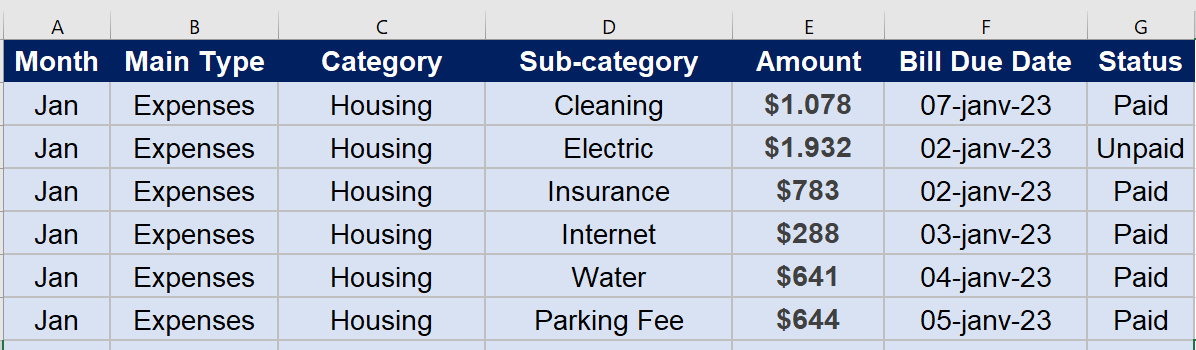
\includegraphics[width=6.0in, height=3.0in]{Figure/Capture d’écran (504).png}
    \caption{Excel raw data}
    \label{fig:enter-label}
\end{figure}

\textbf{Month:} This column refers to the month in which the financial transaction or activity occurred. It provides a chronological timeline for tracking expenses and income over time.

\textbf{Main type:} This column categorizes the type of financial transaction or activity. It could include both categories incomes and expenses.

\textbf{Category:} This column further categorizes the financial transaction or activity into broader categories such as  under  housing, transportation, food, etc.

\textbf{Sub-category: }This column provides more specific details about the nature of the financial transaction or activity within the broader category. For example, under the housing category, sub-categories could include rent, property taxes, insurance, etc.

\textbf{Amount:} This column records the monetary value associated with the financial transaction or activity. It represents the amount of money spent, earned, saved, invested, or owed.

\textbf{Bills due date: }This column indicates the due date for bills or payments associated with the financial transaction or activity.

Status: This column reflects the current status  of the financial transaction or activity. 

\section {How to upload raw data into Power BI}
To create the personal financial dashboard, I followed these steps to upload my data:

\begin{enumerate}
    \item First, I downloaded and installed Power BI Desktop on my computer.
    \item Once it was installed, I opened the application and followed these steps:
    \begin{enumerate}
        \item I clicked on the "Get Data" button to start importing my data.
        \item I chose "Excel Workbook" as the source of my data.
        \item Then, I browsed my computer to find my raw data file and selected the required sheets.
        \item After selecting the sheets, I clicked on "Transform" to proceed.
        \item This opened the Power Query Editor window where I could review and modify my data.
        \item I made sure to check all data types from each table to ensure accuracy.
        \item Finally, I clicked on "Close \& Apply" to import and apply the changes to my data.
    \end{enumerate}
\end{enumerate}

Now, my base data is ready to be used in Power BI.


\section{Data Analysis Expressions (DAX) }
Data Analysis Expressions (DAX) is a query programming language that is used throughout
Microsoft Power BI for creating calculated columns, measures, and custom tables. It is a
collection of functions, operators, and constants that can be used in a formula, or expression, to
calculate and return one or more values.

\section{ Key feature and DAX Queries}
I have created multiple measures with DAX query:

\begin{enumerate}
    \item \textbf{Visualization of monthly expenses by category:}
\\\ Total Expenses = \text{CALCULATE}([\text{Total Amount}], \text{FILTER}('Main Data', 'Main Data'[Main Type]="Expenses"))
\begin{figure}[h]
    \centering
    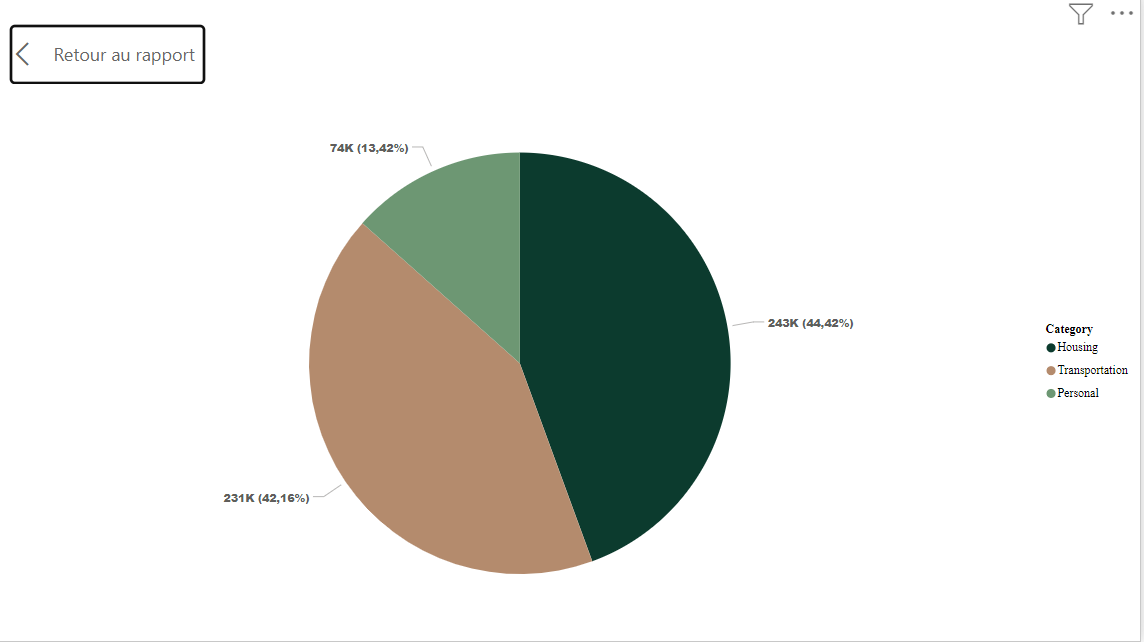
\includegraphics[width=5.0in, height=3.0in]{Figure/expenses-per category.png}
    \caption{Expenses per month by category}
    \label{fig:enter-label}
   
\end{figure}
\\\

 \textbf{ \item {Tracking of monthly income :}}
\text{Total Income} = \text{CALCULATE}([\text{Total Amount}], \text{FILTER}('Main Data', 'Main Data'[Main Type]="Income"))
\\\ 
\text{Side Income} = \text{CALCULATE}([\text{Total Amount}], \text{FILTER}('Main Data', 'Main Data'[Category]="Side Income"))
\\\ 
\text{Main Income} = \text{CALCULATE}([\text{Total Amount}], \text{FILTER}('Main Data', 'Main Data'[Category]="Main Income"))
\begin{figure}[h]
    \centering
    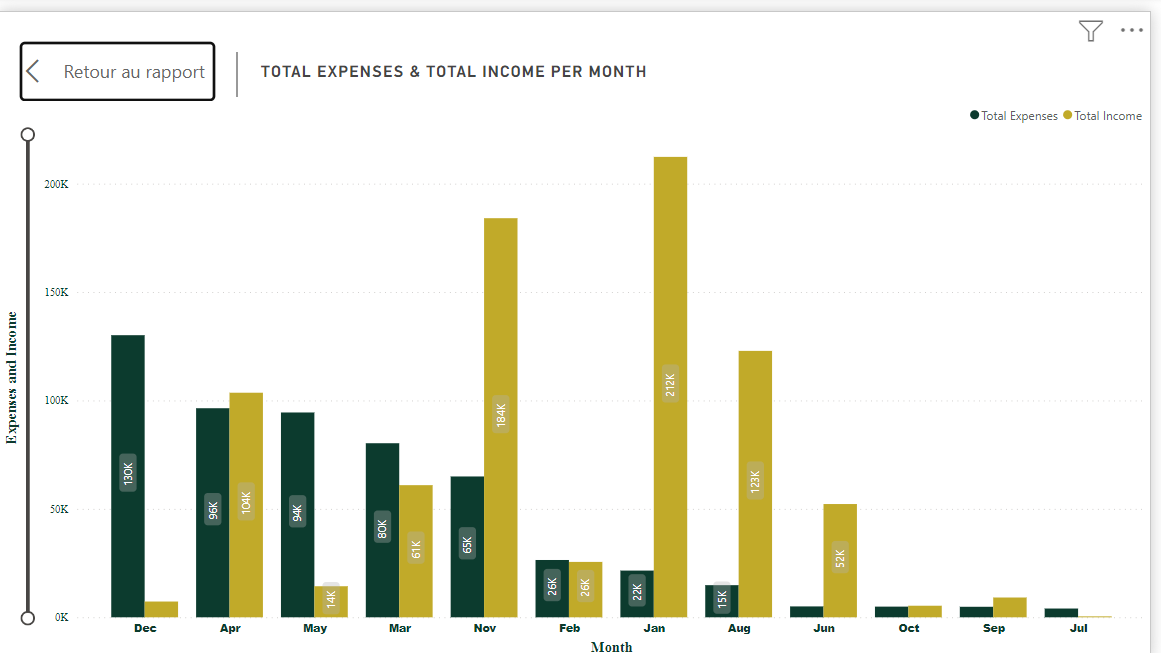
\includegraphics[width=5.0in, height=3.0in]{Figure/expenses-income-per-month.png}
    \caption{Expenses and  income per month}
    \label{fig:enter-label}
   
\end{figure} 


 \item \textbf{Analysis of the net evolution of wealth over time:}

\text{Net Wealth} = 
\text{CALCULATE}(
    \text{SUM}('Main data'[Amount]),
    'Main data'[Main type] = "income"
) - 
\text{CALCULATE}(
    \text{SUM}('Main data'[Amount]),
    'Main data'[Main type] = "expenses"
)
\begin{figure}[h]
    \centering
    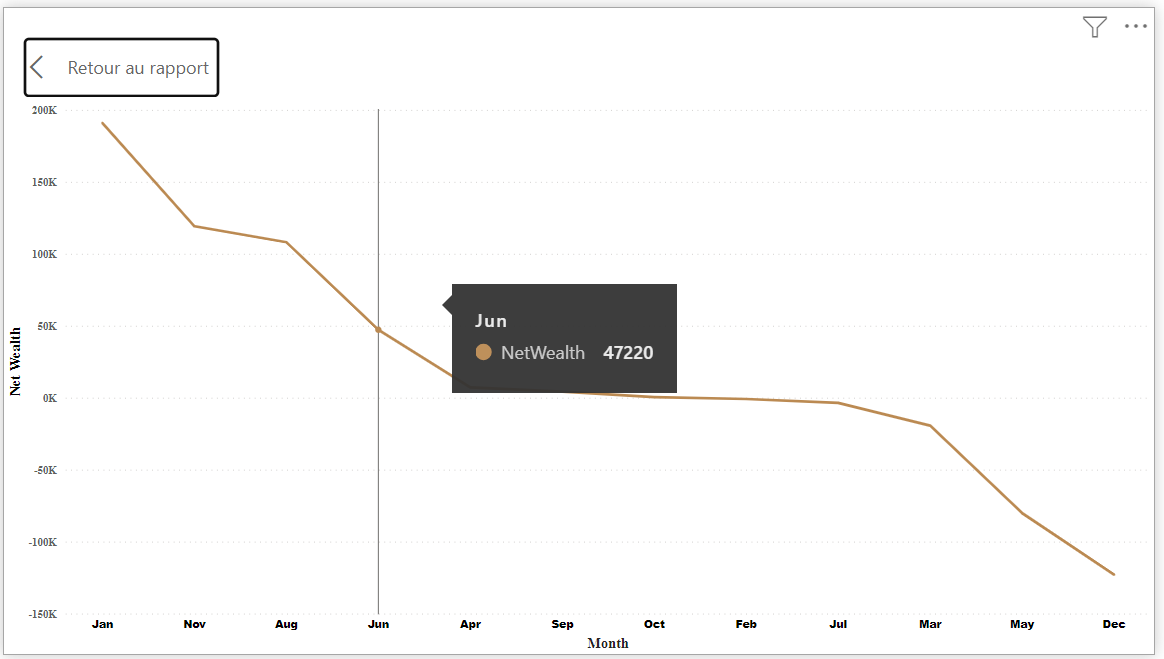
\includegraphics[width=5.0in, height=3.0in]{Figure/Netwealth per month.png}
    \caption{Nat wealth analysis}
    \label{fig:enter-label}
   
\end{figure}












\end{enumerate}





\chapter*{Annex}
\begin{figure}[h]
    \centering
    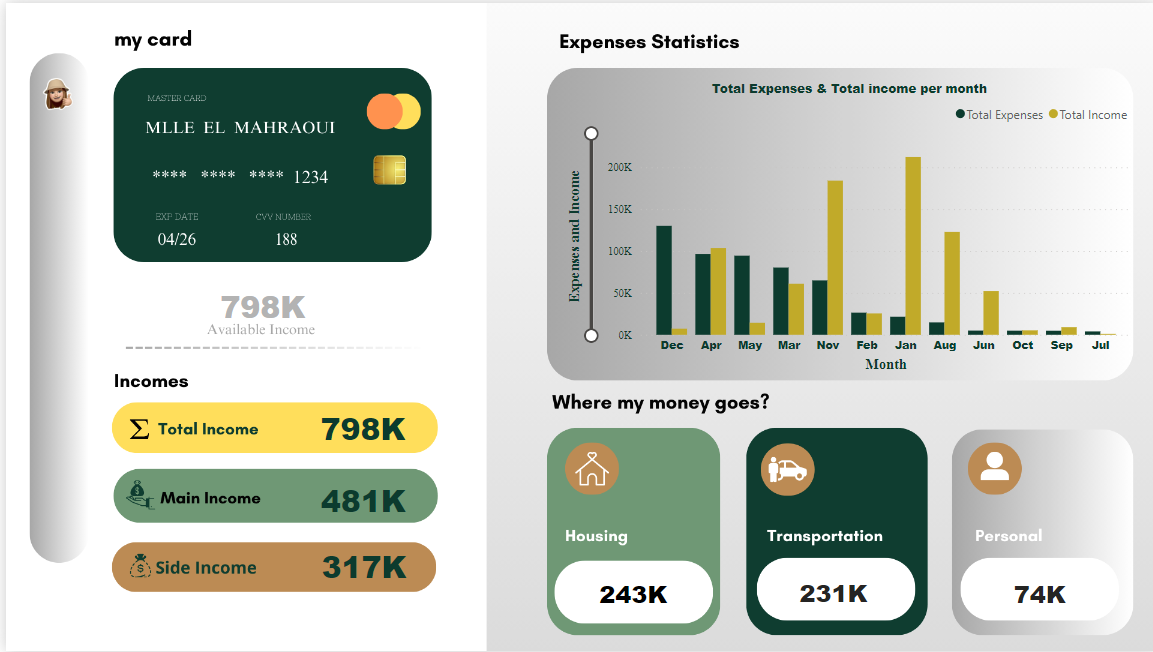
\includegraphics[width=5.0in, height=3.0in]{Figure/Overview (2).png}
    \caption{Dashboard : Page 1}
    \label{fig:enter-label}
   
\end{figure} 

\begin{figure}[h]
    \centering
    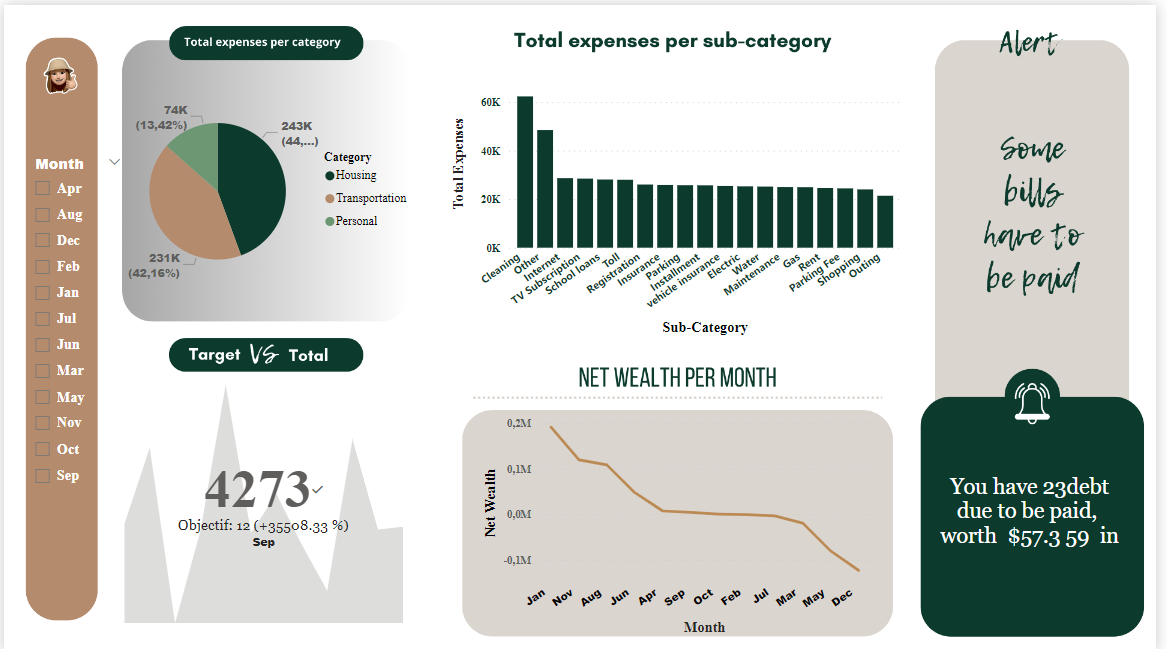
\includegraphics[width=5.0in, height=3.0in]{Figure/visualisation.png}
    \caption{Dashboard : Page 2}
    \label{fig:enter-label}
   
\end{figure} 


\bibliographystyle{plain}
\bibliography{bib}
 \cite{techtarget, sqlspreads}.












\end{document}
